\documentclass[10pt,presentation]{beamer}
\usepackage[spanish]{babel}
\usepackage[utf8]{inputenc}
\usepackage{minted}
\usepackage{datetime}
\newdate{date}{21}{12}{2015}
\date{\displaydate{date}}

\usepackage{booktabs} 
\newcommand{\quotes}[1]{``#1''}

\AtBeginSection[]
{
  \begin{frame}<beamer>
    \frametitle{Outline}
    \tableofcontents[
  currentsection,
  sectionstyle=show/show,
  subsectionstyle=show/shaded/hide
]
  \end{frame}
}

\usepackage{tikz}
\usetikzlibrary{trees}
\usepackage{smartdiagram}

\tikzstyle{every node}=[draw=black,thick,anchor=west]
\tikzstyle{selected}=[draw=red,fill=red!30]
\tikzstyle{optional}=[dashed,fill=gray!50]

\newcommand\TBox[2][]{%
  \tikz\node[draw,ultra thick,align=left,#1] {#2};\hskip2pt}


\title{Conversión de modelos PowerDEVS al lenguaje Modelica} 

\author{Luciano Andrade} 
\institute[UNR] 
{
Universidad Nacional de Rosario\\
\medskip
\textit{andrade.luciano@gmail.com}
}
\date{\displaydate{date}}

\begin{document}

\begin{frame}
\titlepage % Print the title page as the first slide
\end{frame}

\section{Introducción}
	\subsection{Resumen}
%%%%%%%%%%%%%%%%%%%%%%%%%%%%%%%%%%%%%%%%%%%%%%%%%%%%%%%%%%%%%%%%%%%%%%%%%%%%%%%
\begin{frame}{Resumen}
\begin{block}{El modelado y simulación}
son utilizados en el análisis de sistemas  ayudándonos a ganar un mejor entendimiento de su funcionamiento. 
\end{block}

\begin{block}{PowerDEVS}
PowerDEVS es un entorno integrado para el modelado y simulación basado en el formalismo DEVS
\end{block}

\begin{block}{QSS-Solver}
es una implementación independiente de los métodos de integración QSS para simulaciones de sistemas continuos e híbridos. 
\end{block}


\begin{block}{En este trabajo}
se presenta una aplicación capaz de convertir modelos, en PowerDEVS en modelos Modelica, más específicamente $\mu$-Modelica, permitiendo ejecutar este en \quotes{QSS Solver}, lo cual esperamos nos permitá ganar al menos un orden de magnitud en los tiempos incurridos en la simulación.
\end{block}
\end{frame}
%%%%%%%%%%%%%%%%%%%%%%%%%%%%%%%%%%%%%%%%%%%%%%%%%%%%%%%%%%%%%%%%%%%%%%%%%%%%%%%

	\subsection{Motivación}
%%%%%%%%%%%%%%%%%%%%%%%%%%%%%%%%%%%%%%%%%%%%%%%%%%%%%%%%%%%%%%%%%%%%%%%%%%%%%%%
\begin{frame}{Motivación}
\begin{itemize}
	\item<1-> El sistema físico no se encuentra construido. 
	
	\item<2-> El experimento puede ser peligroso. Se realizan simulaciones para determinar si el experimento real \quotes{explotará}.

	\item<3-> El costo del experimento es demasiado alto o las herramientas necesarias no se encuentran disponibles o son muy costosas.

	\item<4-> Los tiempos del sistema no son compatibles con los tiempos del experimentador, ya sea porque es demasiado rápido o porque es demasiado lento.

	\item<5-> Variables de control, de estado y/o del sistema pueden no ser accesibles. Las simulaciones también nos permite manipular el modelo en formas que no podríamos manipular el sistema real.

	\item<6-> Eliminación de perturbaciones. Lo que nos permite aislar efectos particulares, y puede conducir a mejores apreciaciones sobre el comportamiento general del sistema.

	\item<7-> Eliminación de efectos de segundo orden (como no linealidades de componentes del sistema). 
\end{itemize}
\end{frame}
%%%%%%%%%%%%%%%%%%%%%%%%%%%%%%%%%%%%%%%%%%%%%%%%%%%%%%%%%%%%%%%%%%%%%%%%%%%%%%%

	\subsection{Esquema de conversiones}

%%%%%%%%%%%%%%%%%%%%%%%%%%%%%%%%%%%%%%%%%%%%%%%%%%%%%%%%%%%%%%%%%%%%%%%%%%%%%%%
\begin{frame}{Esquema de conversiones}
\begin{figure}
\centering
 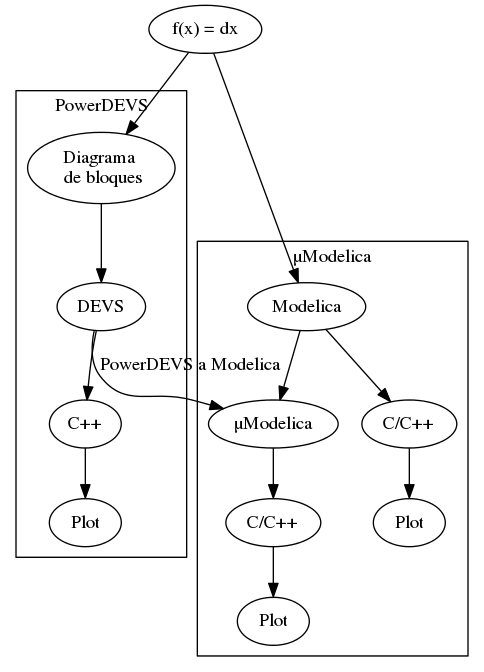
\includegraphics[width=.60\linewidth]{esquema}
\end{figure}
\end{frame}
%%%%%%%%%%%%%%%%%%%%%%%%%%%%%%%%%%%%%%%%%%%%%%%%%%%%%%%%%%%%%%%%%%%%%%%%%%%%%%%

\section{Conceptos Previos}
	\subsection{Modelado y Simulación}
\begin{frame}
\begin{block}{El Modelado y Simulación}
de un sistema es el proceso por el cual se desarrolla un modelo, el cual es luego ejecutado, de forma de obtener datos sobre el comportamiento del sistema. El modelo debe conservar las principales características del sistema, pero al mismo tiempo ser significativamente más simple, de forma que al momento de simularlo sea más eficaz utilizar la simulación que el sistema en sí.
\end{block}
\end{frame}

%%%%%%%%%%%%%%%%%%%%%%%%%%%%%%%%%%%%%%%%%%%%%%%%%%%%%%%%%%%%%%%%%%%%%%%%%%%%%%%
\begin{frame}{Sistemas Continuos y Discretos}
	\begin{equation*} 
	\dot{x}(t) = f (x(t), u(t))
	\end{equation*}
	Con condiciones iniciales :
	\begin{equation*}
	x(t = t_0 ) = x_0
	\end{equation*}

	Si $f$ es continua puede ser aproximada mediante series de Taylor:
	\begin{equation*}
		x_i(t^* + h) = x_i(t^*) + \frac{dx_i (t^*)}{dt} \cdot h + \frac{d^{2}x_i (t^*)}{dt^2} \cdot \frac{h^2}{2!} + \cdots
	\end{equation*}

	\begin{equation*}
		x_i(t^* + h) = x_i(t^*) + f_i(t^*) \cdot h + \frac{d^{2}x_i (t^*)}{dt^2} \cdot \frac{h^2}{2!} + \cdots
	\end{equation*}


\end{frame}
%%%%%%%%%%%%%%%%%%%%%%%%%%%%%%%%%%%%%%%%%%%%%%%%%%%%%%%%%%%%%%%%%%%%%%%%%%%%%%%

	\subsection{Un ejemplo}

%%%%%%%%%%%%%%%%%%%%%%%%%%%%%%%%%%%%%%%%%%%%%%%%%%%%%%%%%%%%%%%%%%%%%%%%%%%%%%%
\begin{frame}{Un ejemplo - Lotka Volterra}
	\begin{align*}
		\frac{dx}{dt} &= x(\alpha - \beta y) \\
		\frac{dy}{dt} &= - y(\gamma - \delta  x)
	\end{align*}
	donde:
	\begin{itemize}
		\item $y$ es el número de algún predador (por ejemplo, un lobo)
		\item $x$ es el número de sus presas (por ejemplo, conejos)
		\item $\frac{dy}{dt}$ y $\frac{dx}{dt}$ representa el crecimiento de las dos poblaciones en el tiempo
		\item $t$ representa el tiempo 
		\item $\alpha$, $\beta$, $\gamma$ y $\delta$ son parámetros que representan las interacciones de las dos especies.
	\end{itemize}
\end{frame}
%%%%%%%%%%%%%%%%%%%%%%%%%%%%%%%%%%%%%%%%%%%%%%%%%%%%%%%%%%%%%%%%%%%%%%%%%%%%%%%

	\subsection{Modelica}

%%%%%%%%%%%%%%%%%%%%%%%%%%%%%%%%%%%%%%%%%%%%%%%%%%%%%%%%%%%%%%%%%%%%%%%%%%%%%%%
\begin{frame}{Modelica}
	\begin{block}{Modelica}
es un lenguaje orientado a objetos desarrollado para describir de manera sencilla modelos de sistemas dinámicos eventualmente muy complejos.
	
\end{block}
\end{frame}
%%%%%%%%%%%%%%%%%%%%%%%%%%%%%%%%%%%%%%%%%%%%%%%%%%%%%%%%%%%%%%%%%%%%%%%%%%%%%%%

%%%%%%%%%%%%%%%%%%%%%%%%%%%%%%%%%%%%%%%%%%%%%%%%%%%%%%%%%%%%%%%%%%%%%%%%%%%%%%%
\begin{frame}[fragile]{Modelica - Modelo Lotka Volterra}
\begin{center}
\begin{figure}[H]    
	\inputminted[linenos]{modelica}{src/LotkaVolterra.mo}
\end{figure}
\end{center}
\end{frame}
%%%%%%%%%%%%%%%%%%%%%%%%%%%%%%%%%%%%%%%%%%%%%%%%%%%%%%%%%%%%%%%%%%%%%%%%%%%%%%%

	\subsection{Métodos de Integración QSS}

%%%%%%%%%%%%%%%%%%%%%%%%%%%%%%%%%%%%%%%%%%%%%%%%%%%%%%%%%%%%%%%%%%%%%%%%%%%%%%%
\begin{frame}{Métodos de Integración QSS}
\begin{block}{El método QSS}
	de primer orden (llamado QSS1) aproxima la ecuación por:
	
	\begin{equation*}
	\dot{x}(t) = f (q(t), v(t))
	\end{equation*}
	
	donde $q$ es el vector de estados cuantificados y sus componentes están relacionadas una a una con las del vector de estados $x$ siguiendo una 
	función de cuantificación con histéresis:
	
	\begin{equation*}
	q_j(t) = \left\{ 
	  \begin{array}{l l}
	    x_j(t)  \quad \text{si} \mid x_j (t ) - q_j (t^{-} ) \mid \geq \Delta Q_j \\
	    q_j (t^{-} ) \quad \text{en caso contrario}
	  \end{array} \right.
	\end{equation*}
	
	donde $q_j (t^{-})$ es el límite por izquierda de $q_j$ en $t$.
\end{block}
\end{frame}
%%%%%%%%%%%%%%%%%%%%%%%%%%%%%%%%%%%%%%%%%%%%%%%%%%%%%%%%%%%%%%%%%%%%%%%%%%%%%%%


%%%%%%%%%%%%%%%%%%%%%%%%%%%%%%%%%%%%%%%%%%%%%%%%%%%%%%%%%%%%%%%%%%%%%%%%%%%%%%%
\begin{frame}{Métodos de Integración QSS}
	  Variables Relacionadas con una Función de Cuantificación con Histéresis de orden cero.
	\begin{figure}[H]
	  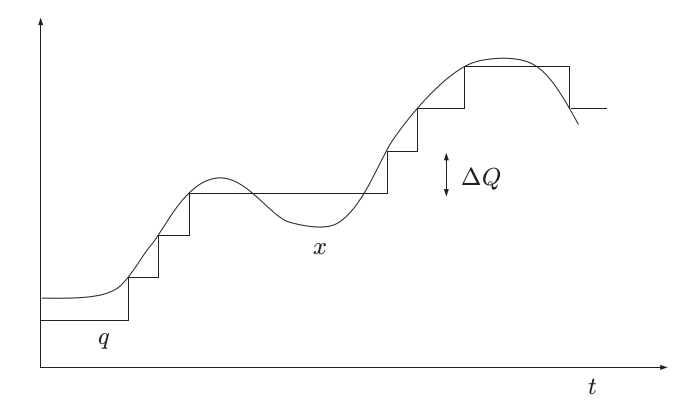
\includegraphics[scale=0.35]{histeresis1}
	\end{figure}
\end{frame}
%%%%%%%%%%%%%%%%%%%%%%%%%%%%%%%%%%%%%%%%%%%%%%%%%%%%%%%%%%%%%%%%%%%%%%%%%%%%%%%

	\subsection{$\mu$-Modelica}

%%%%%%%%%%%%%%%%%%%%%%%%%%%%%%%%%%%%%%%%%%%%%%%%%%%%%%%%%%%%%%%%%%%%%%%%%%%%%%%
\begin{frame}{$\mu$-Modelica}

\begin{block}{La especificación de }
$\mu$-Modelica está basado en la espeficación de Modelica y contiene solo las palabra claves y estructuras necesarias para definir modelos híbridos basados en ODE.
\end{block}
\end{frame}
%%%%%%%%%%%%%%%%%%%%%%%%%%%%%%%%%%%%%%%%%%%%%%%%%%%%%%%%%%%%%%%%%%%%%%%%%%%%%%%

%%%%%%%%%%%%%%%%%%%%%%%%%%%%%%%%%%%%%%%%%%%%%%%%%%%%%%%%%%%%%%%%%%%%%%%%%%%%%%%
\begin{frame}{$\mu$-Modelica}
	\begin{itemize}
	 \item<1-> El modelo es plano, es decir no permite clases.
	 \item<2-> Todas las variables pertenecen al tipo predefinido Real y solo hay tres categorías de variables: estado continuo, estado discreto y variables 
	algebraicas.
	 \item<3-> Los parámetros también son de tipo Real. 
	 \item<4-> Solo Arreglos unidimensionales están permitidos. 
	 \end{itemize}
\end{frame}
%%%%%%%%%%%%%%%%%%%%%%%%%%%%%%%%%%%%%%%%%%%%%%%%%%%%%%%%%%%%%%%%%%%%%%%%%%%%%%%

%%%%%%%%%%%%%%%%%%%%%%%%%%%%%%%%%%%%%%%%%%%%%%%%%%%%%%%%%%%%%%%%%%%%%%%%%%%%%%%
\begin{frame}{$\mu$-Modelica}
	 \begin{itemize}
	 \item<1-> Discontinuidades son expresadas solo con las clausulas $when$ y $elsewhen$ dentro de la sección $algorithm$. Las condiciones dentro de las dos 
	clausulas solo pueden ser relaciones ($<$, $\leqslant$, $>$ $\geqslant$) y, dentro de la clausula, solo asignaciones de variables discretas y $reinit$ 
	de estados continuos son permitidos.

	\item<2-> Indices en los arreglos dentro de cláusulas \texttt{for} están restringidos a la forma $\alpha \cdot i + \beta$, donde $\alpha$ y $\beta$ son expresiones enteras e \texttt{i} es el índice de la iteración.
	\item<3-> La sección de ecuaciones está compuesta de :
	 \begin{itemize}
		\item Definición de variables de estados : $der(x) =  f (x(t), d, a(t), t);$ ODE en forma explícita
		\item Definición algebraica : $a_2  = g(a_1);$
	 \end{itemize}
	 con la restricción de que cada variable algebraica solo puede depender de variables estado y de variables algebraicas previamente definidas.
	\end{itemize}
\end{frame}
%%%%%%%%%%%%%%%%%%%%%%%%%%%%%%%%%%%%%%%%%%%%%%%%%%%%%%%%%%%%%%%%%%%%%%%%%%%%%%%

%%%%%%%%%%%%%%%%%%%%%%%%%%%%%%%%%%%%%%%%%%%%%%%%%%%%%%%%%%%%%%%%%%%%%%%%%%%%%%%
\begin{frame}{$\mu$-Modelica}
	\inputminted[linenos]{modelica}{slides/lotka_volterra_qss.mo}
\end{frame}
%%%%%%%%%%%%%%%%%%%%%%%%%%%%%%%%%%%%%%%%%%%%%%%%%%%%%%%%%%%%%%%%%%%%%%%%%%%%%%%

	\subsection{Stand–Alone QSS solver}

%%%%%%%%%%%%%%%%%%%%%%%%%%%%%%%%%%%%%%%%%%%%%%%%%%%%%%%%%%%%%%%%%%%%%%%%%%%%%%%
\begin{frame}{Stand-Alone QSS-Solver}

\begin{block}{El Stand-Alone QSS-Solver}
es un entorno de modelado y simulación para sistemas híbridos y continuos.
\end{block}

\begin{block}{Los modelos}
son  descriptos en $\mu$-Modelica
\end{block}
\end{frame}
%%%%%%%%%%%%%%%%%%%%%%%%%%%%%%%%%%%%%%%%%%%%%%%%%%%%%%%%%%%%%%%%%%%%%%%%%%%%%%%

	\subsection{Formalismo DEVS}

%%%%%%%%%%%%%%%%%%%%%%%%%%%%%%%%%%%%%%%%%%%%%%%%%%%%%%%%%%%%%%%%%%%%%%%%%%%%%%%
\begin{frame}{Formalismo DEVS}
\begin{block}{DEVS}
	DEVS es un formalismo para modelar y analizar sistemas de eventos discretos 
\end{block}
\begin{block}{Un modelo DEVS}
 puede ser visto como un autómata que procesa una serie de eventos de entrada y genera una serie de eventos de salida y está descripto por dos clases de componentes, modelos atómicos y modelos acoplados.
\end{block}
\end{frame}
%%%%%%%%%%%%%%%%%%%%%%%%%%%%%%%%%%%%%%%%%%%%%%%%%%%%%%%%%%%%%%%%%%%%%%%%%%%%%%%
		\subsubsection{Modelos Atómicos}

%%%%%%%%%%%%%%%%%%%%%%%%%%%%%%%%%%%%%%%%%%%%%%%%%%%%%%%%%%%%%%%%%%%%%%%%%%%%%%%
\begin{frame}{Formalismo DEVS - Modelos Atómicos}
\begin{block}{Un modelo Atómico} 
	representa la unidad \quotes{indivisible} de especificación, en el sentido que es la pieza fundamental y más básica de un modelo DEVS. 
\end{block}
\end{frame}
%%%%%%%%%%%%%%%%%%%%%%%%%%%%%%%%%%%%%%%%%%%%%%%%%%%%%%%%%%%%%%%%%%%%%%%%%%%%%%%

%%%%%%%%%%%%%%%%%%%%%%%%%%%%%%%%%%%%%%%%%%%%%%%%%%%%%%%%%%%%%%%%%%%%%%%%%%%%%%%
\begin{frame}{Formalismo DEVS - Modelos Atómicos}
	Formalmente un modelo atómico está conformado por la 7-upla:

	\begin{equation*} 
	(X, Y, S, \delta_{int} , \delta_{ext}, \lambda, t_{a}) \mbox{ donde :}
	\end{equation*}

	\begin{itemize}
	\item<1-> $X$ es el conjunto de valores de entrada que acepta el modelo atómico.
	\item<2-> $Y$ es el conjunto de valores de los eventos de salida que puede emitir el modelo atómico.
	\item<3-> $S$ es el conjunto de estados internos del modelo.
	\item<4-> $ta$ es una función $S \to \mathbb{R}^{+}_{0}$ de \emph{Avance de Tiempo}.
	\item<5-> $\delta_{int}$ es una función $S \to S$ de \emph{Transición Interna}.
	\item<6-> $\delta_{ext}$ es una función $(S \times \mathbb{R}^{+}_{0} \times X) \to S$ de \emph{Transición Externa}.
	\item<7-> $\lambda$ es una función $S \to Y$ de \emph{Salida}.
	\end{itemize}
\end{frame}
%%%%%%%%%%%%%%%%%%%%%%%%%%%%%%%%%%%%%%%%%%%%%%%%%%%%%%%%%%%%%%%%%%%%%%%%%%%%%%%

%%%%%%%%%%%%%%%%%%%%%%%%%%%%%%%%%%%%%%%%%%%%%%%%%%%%%%%%%%%%%%%%%%%%%%%%%%%%%%%
\begin{frame}{Formalismo DEVS - Modelos Atómicos}
	\begin{figure}[H]
	  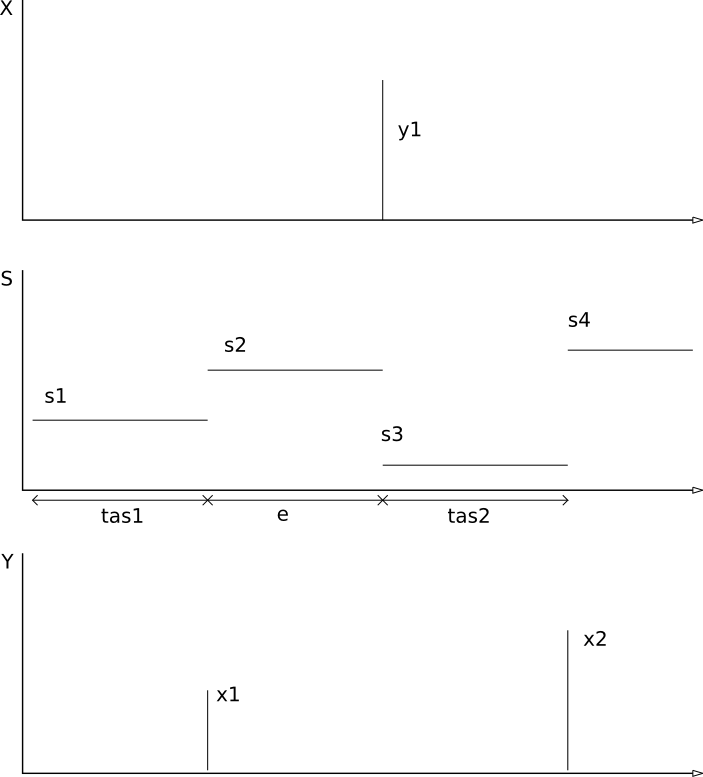
\includegraphics[width=0.6\textwidth]{devs-atomic}
	\end{figure}
\end{frame}
%%%%%%%%%%%%%%%%%%%%%%%%%%%%%%%%%%%%%%%%%%%%%%%%%%%%%%%%%%%%%%%%%%%%%%%%%%%%%%%

		\subsubsection{Modelos Acoplados}

%%%%%%%%%%%%%%%%%%%%%%%%%%%%%%%%%%%%%%%%%%%%%%%%%%%%%%%%%%%%%%%%%%%%%%%%%%%%%%%
\begin{frame}[fragile]{Modelo Acoplados}
	\begin{minipage}{0.48\textwidth}
	\centering
\scalebox{0.75}{%
	\TBox{%
	  \TBox[]{Acoplado2 \\ \TBox{Acoplado1 \\ \TBox[]{Atómico1}\TBox{Atómico2} } \TBox{Atómico3} }}}
	\end{minipage}\hfill\begin{minipage}{0.48\textwidth}
	\centering
\scalebox{0.75}{%
	\begin{tikzpicture}[%
	  grow via three points={one child at (0.5,-0.7) and
	  two children at (0.5,-0.7) and (0.5,-1.4)},
	  edge from parent path={(\tikzparentnode.south) |- (\tikzchildnode.west)}]
	  \node {Root-Coordinator}
	    child { node {Acoplado2}		
	    child { node {Acoplado1}
	      child { node {Atómico1}}
	      child { node {Atómico2}}
	    }
	    child [missing] {}				
	    child [missing] {}				
	    child [missing] {}				
	    child { node {Atómico3}}};
	\end{tikzpicture}
}
	\end{minipage}
\end{frame}
%%%%%%%%%%%%%%%%%%%%%%%%%%%%%%%%%%%%%%%%%%%%%%%%%%%%%%%%%%%%%%%%%%%%%%%%%%%%%%%

		\subsubsection{Modelos Vectoriales}

%%%%%%%%%%%%%%%%%%%%%%%%%%%%%%%%%%%%%%%%%%%%%%%%%%%%%%%%%%%%%%%%%%%%%%%%%%%%%%%
\begin{frame}{Modelos Vectoriales}
\begin{block}{Modelos Vectoriales}
Nos permiten especificar un vector de Modelos y facilita el modelado de grandes sistemas.
\end{block}
\centering
\begin{block}{StateChart de un modelo Vectorial}
\begin{center}
\begin{figure}
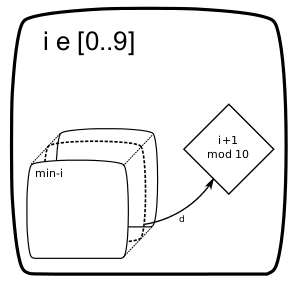
\includegraphics[width=.40\linewidth]{img/statechart.png}
\end{figure}
\end{center}
\end{block}
\end{frame}
%%%%%%%%%%%%%%%%%%%%%%%%%%%%%%%%%%%%%%%%%%%%%%%%%%%%%%%%%%%%%%%%%%%%%%%%%%%%%%%

	\subsection{PowerDEVS}

%%%%%%%%%%%%%%%%%%%%%%%%%%%%%%%%%%%%%%%%%%%%%%%%%%%%%%%%%%%%%%%%%%%%%%%%%%%%%%%
\begin{frame}{PowerDEVS}
\begin{block}{PowerDEVS} 
 es un programa, concebido para ser utilizado por expertos programadores DEVS, así como usuarios finales que solo quieren 
	conectar bloques y simular.
\end{block}
\end{frame}
%%%%%%%%%%%%%%%%%%%%%%%%%%%%%%%%%%%%%%%%%%%%%%%%%%%%%%%%%%%%%%%%%%%%%%%%%%%%%%%

%%%%%%%%%%%%%%%%%%%%%%%%%%%%%%%%%%%%%%%%%%%%%%%%%%%%%%%%%%%%%%%%%%%%%%%%%%%%%%%
\begin{frame}{PowerDEVS}
	\begin{figure}[H]
	  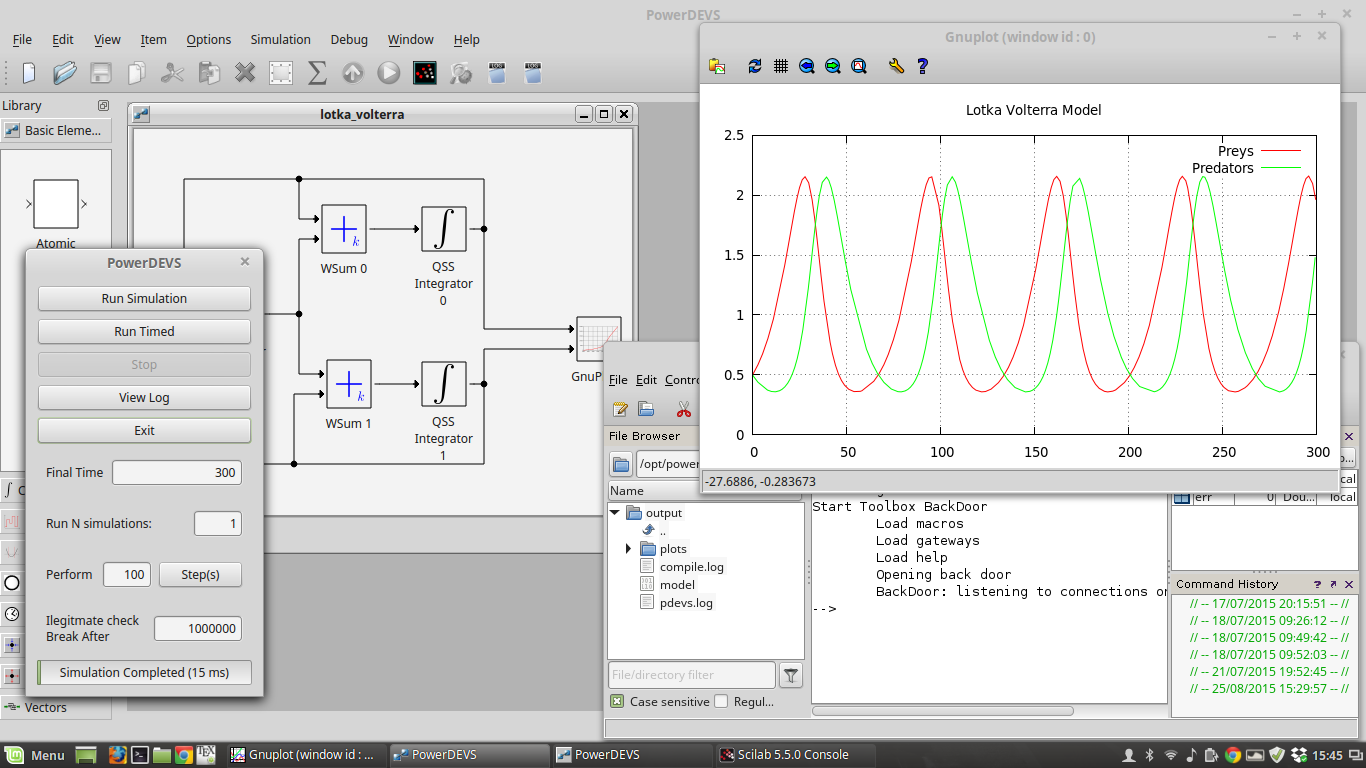
\includegraphics[width=\textwidth]{powerdevs}
	\end{figure}
\end{frame}
%%%%%%%%%%%%%%%%%%%%%%%%%%%%%%%%%%%%%%%%%%%%%%%%%%%%%%%%%%%%%%%%%%%%%%%%%%%%%%%

%%%%%%%%%%%%%%%%%%%%%%%%%%%%%%%%%%%%%%%%%%%%%%%%%%%%%%%%%%%%%%%%%%%%%%%%%%%%%%%
\begin{frame}{PowerDEVS - Modelo Lotka Volterra}
\centering
\begin{figure}[H]
	  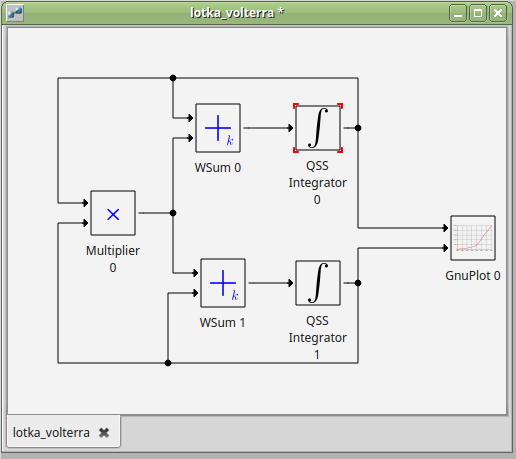
\includegraphics[width=0.7\textwidth]{lk-powerdevs}
\end{figure}
\end{frame}
%%%%%%%%%%%%%%%%%%%%%%%%%%%%%%%%%%%%%%%%%%%%%%%%%%%%%%%%%%%%%%%%%%%%%%%%%%%%%%%

\section{Conversión de modelos DEVS}
	\subsection{Modelos DEVS}
%%%%%%%%%%%%%%%%%%%%%%%%%%%%%%%%%%%%%%%%%%%%%%%%%%%%%%%%%%%%%%%%%%%%%%%%%%%%%%%
\begin{frame}{Conversión de modelos DEVS}
\begin{block}{PowerDEVS}
	Trabaja principalmente con dos archivos, .PDM y .PDS.
\end{block}
\begin{itemize}
        \item<1-> Los archivos PDM son utilizados por el editor de PowerDEVS.
        \item<2-> El archivo PDS contiene información estructural del modelo necesaria para realizar la simulación. 
\end{itemize}
\end{frame}
%%%%%%%%%%%%%%%%%%%%%%%%%%%%%%%%%%%%%%%%%%%%%%%%%%%%%%%%%%%%%%%%%%%%%%%%%%%%%%%
		\subsubsection{Archivos PDS}

%%%%%%%%%%%%%%%%%%%%%%%%%%%%%%%%%%%%%%%%%%%%%%%%%%%%%%%%%%%%%%%%%%%%%%%%%%%%%%%
\begin{frame}[fragile]{Archivos PDS}
\begin{minted}{text}
...
  Simulator
   {
    Path = qss/qss_integrator.h
    Parameters = "QSS3","1e-6","1e-3","0.5"
   }
 
...
\end{minted}
\end{frame}
%%%%%%%%%%%%%%%%%%%%%%%%%%%%%%%%%%%%%%%%%%%%%%%%%%%%%%%%%%%%%%%%%%%%%%%%%%%%%%%

%%%%%%%%%%%%%%%%%%%%%%%%%%%%%%%%%%%%%%%%%%%%%%%%%%%%%%%%%%%%%%%%%%%%%%%%%%%%%%%
\begin{frame}[fragile]{QSSIntegrator}
\centering
    qss/qss\_integrator.mo
\begin{minted}{modelica}
class QSSIntegrator
  parameter Real p[4]={0,0,0,0};
  parameter Real x0 = p[4];
  Real u[1];
  Real y[1](start = {x0});
equation
  der(y[1]) = u[1];
end QSSIntegrator;
\end{minted}
\end{frame}
%%%%%%%%%%%%%%%%%%%%%%%%%%%%%%%%%%%%%%%%%%%%%%%%%%%%%%%%%%%%%%%%%%%%%%%%%%%%%%%

%%%%%%%%%%%%%%%%%%%%%%%%%%%%%%%%%%%%%%%%%%%%%%%%%%%%%%%%%%%%%%%%%%%%%%%%%%%%%%%
\begin{frame}[fragile]{Archivos PDS}
\centering
\begin{minted}{modelica}
class QSSIntegrator
  parameter Real QSSIntegrator_1_p[4]={0,1e-6, 1e-3, 0.5};
  parameter Real QSSIntegrator_1_x0 = p[4];
  Real QSSIntegrator_1_u[1];
  Real QSSIntegrator_1_y[1](start = {QSSIntegrator_1_x0});
equation
  der(QSSIntegrator_1_y[1]) = QSSIntegrator_1_u[1];
end QSSIntegrator;
\end{minted}
\end{frame}
%%%%%%%%%%%%%%%%%%%%%%%%%%%%%%%%%%%%%%%%%%%%%%%%%%%%%%%%%%%%%%%%%%%%%%%%%%%%%%%

		\subsubsection{Protocolo}
%%%%%%%%%%%%%%%%%%%%%%%%%%%%%%%%%%%%%%%%%%%%%%%%%%%%%%%%%%%%%%%%%%%%%%%%%%%%%%%
\begin{frame}[fragile]{Protocolo}
\begin{itemize}
        \item<1-> El código debe ser Modelica ($\mu$-Modelica) válido y estar ubicado en el mismo directorio (y nombre del archivo) del código C que el modelo atómico 
        PowerDEVS, con el mismo nombre que el archivo .h, pero con extensión .mo, es decir un modelo con \texttt{vector\textbackslash qss\_sum\_vec.h} 
	utilizará un modelo \texttt{vector/qss\_sum\_vec.h} 
        \item<2-> Los parámetros del modelo DEVS deben ser pasado en el parámetro $p$, el cual es un arreglo de reales. 
        \item<3-> Los valores de entrada son asociados a la variable $u$
        \item<4-> Los valores de salida son asociados a la variable $y$
\end{itemize}
\end{frame}
%%%%%%%%%%%%%%%%%%%%%%%%%%%%%%%%%%%%%%%%%%%%%%%%%%%%%%%%%%%%%%%%%%%%%%%%%%%%%%%

	\subsection{Modelos Acoplados Planos}

%%%%%%%%%%%%%%%%%%%%%%%%%%%%%%%%%%%%%%%%%%%%%%%%%%%%%%%%%%%%%%%%%%%%%%%%%%%%%%%
\begin{frame}[fragile]{Modelos Acoplados Planos}
\begin{minted}{modelica}
model lotka_volterra
...
  Real QSSIntegrator_1_u[1];
  Real QSSIntegrator_1_y[1](start = QSSIntegrator_1_x0);
  Real QSSIntegrator_2_u[1];
  Real QSSIntegrator_2_y[1](start = QSSIntegrator_2_x0);
...
equation
...
  qss_multiplier_0_u[1] = QSSIntegrator_1_y[1];
  qss_multiplier_0_u[2] = QSSIntegrator_2_y[1];
  WSum_3_u[1] = QSSIntegrator_1_y[1];
  WSum_4_u[2] = QSSIntegrator_2_y[1];
  der(QSSIntegrator_2_y[1]) = QSSIntegrator_2_u[1];
  der(QSSIntegrator_1_y[1]) = QSSIntegrator_1_u[1];
...
end lotka_volterra;
\end{minted}
\end{frame}
%%%%%%%%%%%%%%%%%%%%%%%%%%%%%%%%%%%%%%%%%%%%%%%%%%%%%%%%%%%%%%%%%%%%%%%%%%%%%%%

	\subsection{Modelos Acoplados Jerárquicos }

%%%%%%%%%%%%%%%%%%%%%%%%%%%%%%%%%%%%%%%%%%%%%%%%%%%%%%%%%%%%%%%%%%%%%%%%%%%%%%%
\begin{frame}[fragile]{Ejemplo de modelo acoplado - Convertidor de Voltaje}
        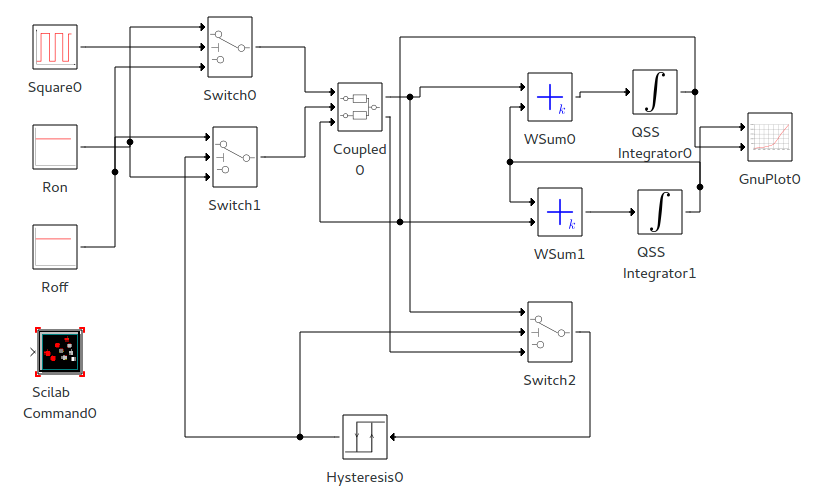
\includegraphics[width=\linewidth]{buck_disk}
\end{frame}
%%%%%%%%%%%%%%%%%%%%%%%%%%%%%%%%%%%%%%%%%%%%%%%%%%%%%%%%%%%%%%%%%%%%%%%%%%%%%%%

%%%%%%%%%%%%%%%%%%%%%%%%%%%%%%%%%%%%%%%%%%%%%%%%%%%%%%%%%%%%%%%%%%%%%%%%%%%%%%%
\begin{frame}{Ejemplo de modelo acoplado - Convertidor de Voltaje - Coupled0}
        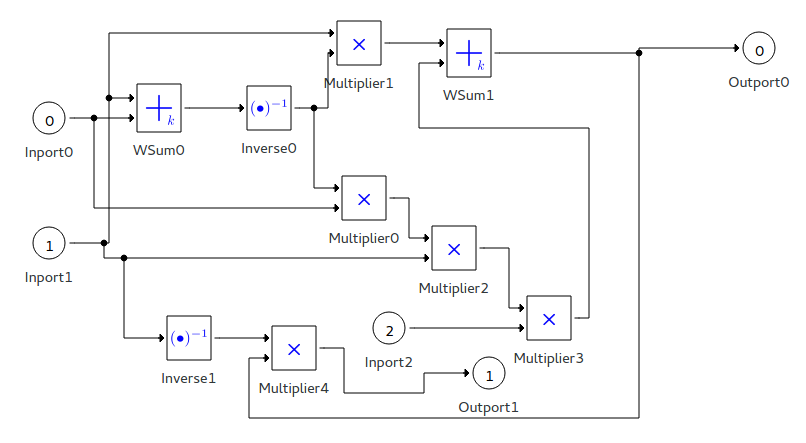
\includegraphics[width=\linewidth]{buck_disk_coupled0}
\end{frame}
%%%%%%%%%%%%%%%%%%%%%%%%%%%%%%%%%%%%%%%%%%%%%%%%%%%%%%%%%%%%%%%%%%%%%%%%%%%%%%%

%%%%%%%%%%%%%%%%%%%%%%%%%%%%%%%%%%%%%%%%%%%%%%%%%%%%%%%%%%%%%%%%%%%%%%%%%%%%%%%
\begin{frame}[fragile]{Convertidor de Voltaje}
\begin{figure}[H]
  %\setcapwidth{0.6\textwidth}
        \begin{minipage}[t][][b]{.40\textwidth}
\centering	Jerárquico \\
\scalebox{0.45}{%
        \begin{tikzpicture}[%
          grow via three points={one child at (0.5,-0.7) and
          two children at (0.5,-0.7) and (0.5,-1.4)},
          edge from parent path={(\tikzparentnode.south) |- (\tikzchildnode.west)}]
          \node {Root-Coordinator}
            child { node (R1) {Scilab Command0 (1)}}
            child { node (R2) {QSS Integartor0 (2)}}
            child { node (R3) {QSS Integartor1 (3)}}             
            child { node (R4) {Coupled0        (4)}
              child { node (C1) {WSum0       (1)}}
              child { node (C2) {Inseverse0  (2)}}
              child { node (C3) {Multiplier0 (3)}}
              child { node (C4) {Multiplier1 (4)}}
              child { node (C5) {Multiplier2 (5)}}
              child { node (C6) {Inseverse1  (6)}}
              child { node (C7) {Multiplier3 (7)}}
              child { node (C8) {Multiplier4 (8)}}
              child { node (C9) {WSum1       (9)}}
            }
            child [missing] {}                          
            child [missing] {}                          
            child [missing] {}                          
            child [missing] {}                          
            child [missing] {}                          
            child [missing] {}                          
            child [missing] {}                          
            child [missing] {}                          
            child [missing] {}                          
            child { node (R5) {Switch0    (5)}}
            child { node (R6) {Ron        (6)}}
            child { node (R7) {Roff       (7)}}
            child { node (R8) {Square0    (8)}}
            child { node (R9) {GNUPlot0   (9)}}
            child { node (R10) {Hysteresis0(10)}}
            child { node (R11) {Switch1    (11)}}
            child { node (R12) {WSum0      (12)}}
            child { node (R13) {WSum1      (13)}};
        \end{tikzpicture}
}
        \end{minipage} \hfill \begin{minipage}[t][][b]{.40\textwidth}
\centering Plano \\
\scalebox{0.45}{%
        \begin{tikzpicture}[%
          grow via three points={one child at (0.5,-0.7) and
          two children at (0.5,-0.7) and (0.5,-1.4)},
          edge from parent path={(\tikzparentnode.south) |- (\tikzchildnode.west)}]
          \node {Root-Coordinator}
            child { node (1) {Scilab Command0	(1)}}
            child { node (2) {QSS Integartor0	(2)}}
            child { node (3) {QSS Integartor1	(3)}}             
            child { node (4) {WSum0			(4)}}
            child { node (5) {Inseverse0		(5)}}
            child { node (6) {Multiplier0		(6)}}
            child { node (7) {Multiplier1		(7)}}
            child { node (8) {Multiplier2		(8)}}
            child { node (9) {Inseverse1		(9)}}
            child { node (10) {Multiplier3		(10)}}
            child { node (11) {Multiplier4		(11)}}
            child { node (12) {WSum1			(12)}}
            child { node (13) {Switch0			(13)}}
            child { node (14) {Ron			(14)}}
            child { node (15) {Roff			(15)}}
            child { node (16) {Square0		(16)}}
            child { node (17) {GNUPlot0		(17)}}
            child { node (18) {Hysteresis0		(18)}}
            child { node (19) {Switch1		(19)}}
            child { node (20) {WSum0			(20)}}
            child { node (21) {WSum1			(21)}};

        \end{tikzpicture}
}
        \end{minipage}%
\end{figure}
\end{frame}

%%%%%%%%%%%%%%%%%%%%%%%%%%%%%%%%%%%%%%%%%%%%%%%%%%%%%%%%%%%%%%%%%%%%%%%%%%%%%%%

%%%%%%%%%%%%%%%%%%%%%%%%%%%%%%%%%%%%%%%%%%%%%%%%%%%%%%%%%%%%%%%%%%%%%%%%%%%%%%%
\begin{frame}[fragile]{Convertidor de Voltaje}
\begin{figure}[H]
  %\setcapwidth{0.6\textwidth}
        \begin{minipage}[t][][b]{.40\textwidth}
\centering	Jerárquico \\
\scalebox{0.45}{%
        \begin{tikzpicture}[%
          grow via three points={one child at (0.5,-0.7) and
          two children at (0.5,-0.7) and (0.5,-1.4)},
          edge from parent path={(\tikzparentnode.south) |- (\tikzchildnode.west)}]
          \node {Root-Coordinator}
            child { node (R1) {Scilab Command0 (1)}}
            child { node (R2) {QSS Integartor0 (2)}}
            child { node (R3) {QSS Integartor1 (3)}}             
            child { node (R4) {Coupled0        (4)}
              child { node (C1) {WSum0       (1)}}
              child { node (C2) {Inseverse0  (2)}}
              child { node (C3) {Multiplier0 (3)}}
              child { node (C4) {Multiplier1 (4)}}
              child { node (C5) {Multiplier2 (5)}}
              child { node (C6) {Inseverse1  (6)}}
              child { node (C7) {Multiplier3 (7)}}
              child { node (C8) {Multiplier4 (8)}}
              child { node (C9) {WSum1       (9)}}
            }
            child [missing] {}                          
            child [missing] {}                          
            child [missing] {}                          
            child [missing] {}                          
            child [missing] {}                          
            child [missing] {}                          
            child [missing] {}                          
            child [missing] {}                          
            child [missing] {}                          
            child { node (R5) {Switch0    (5)}}
            child { node (R6) {Ron        (6)}}
            child { node (R7) {Roff       (7)}}
            child { node (R8) {Square0    (8)}}
            child { node (R9) {GNUPlot0   (9)}}
            child { node (R10) {Hysteresis0(10)}}
            child { node (R11) {Switch1    (11)}}
            child { node (R12) {WSum0      (12)}}
            child { node (R13) {WSum1      (13)}};
	    \path[->,line width=1pt,red] (C7.east) edge[bend left=90 ] (C8.east);
	    \path[->,line width=1pt,red] (R13.east) edge[bend right=90 ] (R1.east);

	    \path[->,line width=1pt,green] (R3.east) edge[bend left=90 ] (R4.east);
	    \path[->,line width=1pt,green] (R4.east) edge[bend left=90 ] (C4.east);

	    \path[->,line width=1pt,blue] (R6.east) edge[bend right=90] (R4.east);
	    \path[->,line width=1pt,blue] (R4.east) edge[bend left=90] (C8.east);
        \end{tikzpicture}
}
        \end{minipage} \hfill \begin{minipage}[t][][b]{.40\textwidth}
\centering Plano \\
\scalebox{0.45}{%
        \begin{tikzpicture}[%
          grow via three points={one child at (0.5,-0.7) and
          two children at (0.5,-0.7) and (0.5,-1.4)},
          edge from parent path={(\tikzparentnode.south) |- (\tikzchildnode.west)}]
          \node {Root-Coordinator}
            child { node (1) {Scilab Command0	(1)}}
            child { node (2) {QSS Integartor0	(2)}}
            child { node (3) {QSS Integartor1	(3)}}             
            child { node (4) {WSum0			(4)}}
            child { node (5) {Inseverse0		(5)}}
            child { node (6) {Multiplier0		(6)}}
            child { node (7) {Multiplier1		(7)}}
            child { node (8) {Multiplier2		(8)}}
            child { node (9) {Inseverse1		(9)}}
            child { node (10) {Multiplier3		(10)}}
            child { node (11) {Multiplier4		(11)}}
            child { node (12) {WSum1			(12)}}
            child { node (13) {Switch0			(13)}}
            child { node (14) {Ron			(14)}}
            child { node (15) {Roff			(15)}}
            child { node (16) {Square0		(16)}}
            child { node (17) {GNUPlot0		(17)}}
            child { node (18) {Hysteresis0		(18)}}
            child { node (19) {Switch1		(19)}}
            child { node (20) {WSum0			(20)}}
            child { node (21) {WSum1			(21)}};

	    \path[->,line width=1pt,red] (10.east) edge[bend left=90 ] (11.east);
	    \path[->,line width=1pt,red] (21.east) edge[bend right=90 ] (1.east);

	    \path[->,line width=1pt,green] (3.east) edge[bend left=90 ] (7.east);

	    \path[->,line width=1pt,blue] (14.east) edge[bend right=90] (11.east);
        \end{tikzpicture}
}
        \end{minipage}%
\end{figure}
\end{frame}

%%%%%%%%%%%%%%%%%%%%%%%%%%%%%%%%%%%%%%%%%%%%%%%%%%%%%%%%%%%%%%%%%%%%%%%%%%%%%%%

	\subsection{Modelos Vectoriales}

%%%%%%%%%%%%%%%%%%%%%%%%%%%%%%%%%%%%%%%%%%%%%%%%%%%%%%%%%%%%%%%%%%%%%%%%%%%%%%%
\begin{frame}[fragile]{Modelos Vectoriales}
Las conexiones entre modelos vectoriales, deben ser tratadas de forma diferente,
ya que representan un vector de conexiones en lugar de una conexion.

\begin{minted}{modelica}
  for i in 1:1000 loop
    IndexShift_2_u[1][i] = VecInt_1_y[1][i];
  end for;
  for i in 1:1000 loop
    vector_pow2_6_u[1][i] = VecInt_1_y[1][i];
  end for;
  for i in 1:1000 loop
    VectorSum_8_u[2][i] = VecInt_1_y[1][i];
  end for;
\end{minted}
\end{frame}
%%%%%%%%%%%%%%%%%%%%%%%%%%%%%%%%%%%%%%%%%%%%%%%%%%%%%%%%%%%%%%%%%%%%%%%%%%%%%%%

	\subsection{Transformaciones Extras}

%%%%%%%%%%%%%%%%%%%%%%%%%%%%%%%%%%%%%%%%%%%%%%%%%%%%%%%%%%%%%%%%%%%%%%%%%%%%%%%
\begin{frame}{Transformaciones Extras}
\begin{itemize}
	\item<1-> Producto Interno
	\item<2-> Arreglos Bidimensionales
	\item<3-> Condicional
\end{itemize}
\end{frame}
%%%%%%%%%%%%%%%%%%%%%%%%%%%%%%%%%%%%%%%%%%%%%%%%%%%%%%%%%%%%%%%%%%%%%%%%%%%%%%%

%%%%%%%%%%%%%%%%%%%%%%%%%%%%%%%%%%%%%%%%%%%%%%%%%%%%%%%%%%%%%%%%%%%%%%%%%%%%%%%
\begin{frame}[fragile]{Ejemplo Arreglos Bidimensionales}
\begin{block}{Antes}
\begin{minted}[breaklines=true]{modelica}
Real IndexShift_2_u[IndexShift_2_N,2];
\end{minted}
\end{block}

\begin{block}{Después}
\begin{minted}[breaklines=true]{modelica}
Real IndexShift_2_u_1[IndexShift_2_N];
Real IndexShift_2_u_2[IndexShift_2_N];
\end{minted}
\end{block}
\end{frame}
%%%%%%%%%%%%%%%%%%%%%%%%%%%%%%%%%%%%%%%%%%%%%%%%%%%%%%%%%%%%%%%%%%%%%%%%%%%%%%%



%%%%%%%%%%%%%%%%%%%%%%%%%%%%%%%%%%%%%%%%%%%%%%%%%%%%%%%%%%%%%%%%%%%%%%%%%%%%%%%
\begin{frame}[fragile]{Ejemplo de producto Interno}
\begin{block}{Antes}
\begin{minted}[breaklines=true]{modelica}
    VectorSum_3_y_1[VectorSum_3_i] = VectorSum_3_u[VectorSum_3_i, 1:VectorSum_3_nin] * VectorSum_3_w;
\end{minted}
\end{block}
	
\begin{block}{Después}
\begin{minted}[breaklines=true]{modelica}
    VectorSum_3_y[1,VectorSum_3_i] = VectorSum_3_u[1,VectorSum_3_i]*VectorSum_3_w[1]+ VectorSum_3_u[2,VectorSum_3_i]*VectorSum_3_w[2]+ VectorSum_3_u[3,VectorSum_3_i]*VectorSum_3_w[3]+ VectorSum_3_u[4,VectorSum_3_i]*VectorSum_3_w[4];
\end{minted}
\end{block}
\end{frame}
%%%%%%%%%%%%%%%%%%%%%%%%%%%%%%%%%%%%%%%%%%%%%%%%%%%%%%%%%%%%%%%%%%%%%%%%%%%%%%%

%%%%%%%%%%%%%%%%%%%%%%%%%%%%%%%%%%%%%%%%%%%%%%%%%%%%%%%%%%%%%%%%%%%%%%%%%%%%%%%
\begin{frame}[fragile]{Ejemplo Condicional - Antes}
\begin{minted}[breaklines=true]{modelica}
  if IndexShift_2_Shift > 0 then
    for IndexShift_2_i in 1:IndexShift_2_N-IndexShift_2_Shift loop
      IndexShift_2_y_1[IndexShift_2_i+IndexShift_2_Shift] = IndexShift_2_u_1[IndexShift_2_i];
    end for;
    for IndexShift_2_i in 1:IndexShift_2_Shift loop
      IndexShift_2_y_1[IndexShift_2_i] = 0;
    end for;
  else
    for IndexShift_2_i in 1:IndexShift_2_N-IndexShift_2_Shift loop
      IndexShift_2_y_1[IndexShift_2_i] = 
		IndexShift_2_u_1[IndexShift_2_i - +IndexShift_2_Shift];
    end for;
    for IndexShift_2_i in IndexShift_2_N + IndexShift_2_Shift : IndexShift_2_N loop
      IndexShift_2_y_1[IndexShift_2_i] = 0;
    end for;
  end if;
\end{minted}
\end{frame}
%%%%%%%%%%%%%%%%%%%%%%%%%%%%%%%%%%%%%%%%%%%%%%%%%%%%%%%%%%%%%%%%%%%%%%%%%%%%%%%

%%%%%%%%%%%%%%%%%%%%%%%%%%%%%%%%%%%%%%%%%%%%%%%%%%%%%%%%%%%%%%%%%%%%%%%%%%%%%%%
\begin{frame}[fragile]{Ejemplo Condicional - Después}
\begin{minted}[breaklines=true]{modelica}
  for IndexShift_2_i in 1:IndexShift_2_N-IndexShift_2_Shift loop
    IndexShift_2_y_1[IndexShift_2_i+IndexShift_2_Shift] = IndexShift_2_u_1[IndexShift_2_i];
  end for;
  for IndexShift_2_i in 1:IndexShift_2_Shift loop
    IndexShift_2_y_1[IndexShift_2_i] = 0;
  end for;
\end{minted}
\end{frame}
%%%%%%%%%%%%%%%%%%%%%%%%%%%%%%%%%%%%%%%%%%%%%%%%%%%%%%%%%%%%%%%%%%%%%%%%%%%%%%%

\section{Resultados}
	\subsection{Lotka Volterra}
%%%%%%%%%%%%%%%%%%%%%%%%%%%%%%%%%%%%%%%%%%%%%%%%%%%%%%%%%%%%%%%%%%%%%%%%%%%%%%%
\begin{frame}{Resultados - Lotka-Volterra}
\begin{align*}
\frac{dx}{dt} & = x(\alpha - \beta y)\\
\frac{dy}{dt} & =y(\gamma - \delta  x)
\end{align*}

donde:
\begin{itemize}
    \item y es el número de algún predador (por ejemplo, un lobo);
    \item x es el número de sus presas (por ejemplo, conejos);
    \item t representa el tiempo; y
    \item $\alpha$, $\beta$, $\gamma$, $\delta$ son parámetros que representan las interacciones de las dos especies.
\end{itemize}
\end{frame}
%%%%%%%%%%%%%%%%%%%%%%%%%%%%%%%%%%%%%%%%%%%%%%%%%%%%%%%%%%%%%%%%%%%%%%%%%%%%%%%

%%%%%%%%%%%%%%%%%%%%%%%%%%%%%%%%%%%%%%%%%%%%%%%%%%%%%%%%%%%%%%%%%%%%%%%%%%%%%%%
\begin{frame}{Resultados - Lotka-Volterra}
\begin{figure}[H]
\begin{minipage}{0.5\textwidth}
\centering
PowerDEVS \\
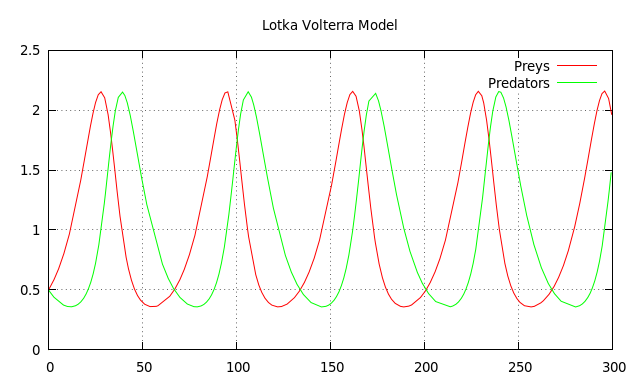
\includegraphics[width=\linewidth]{lotka_volterra-pd}
\end{minipage}\hfill\begin{minipage}{0.5\textwidth}
\centering
QSS-Solver \\
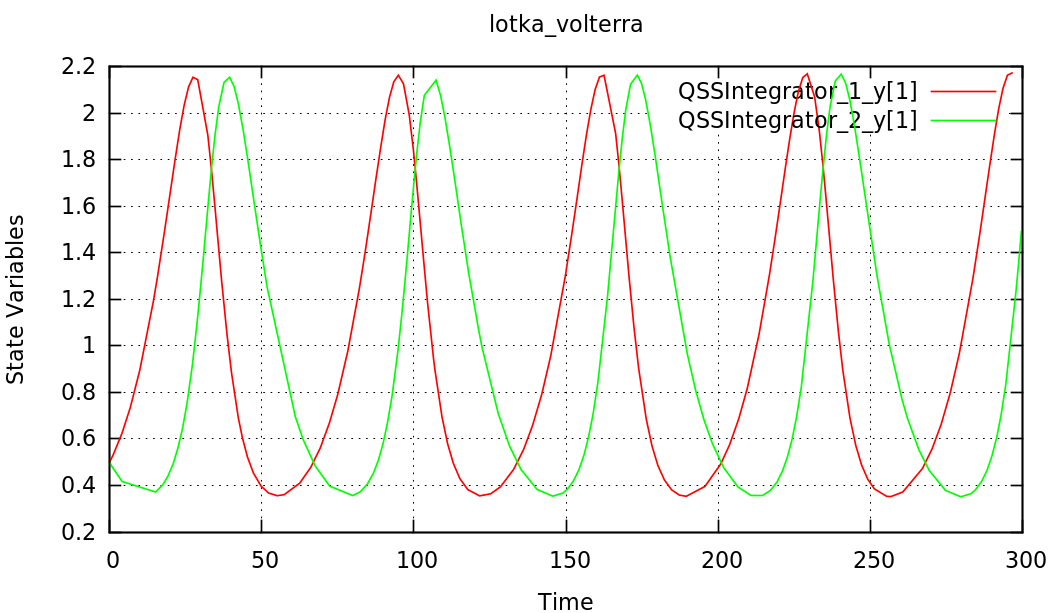
\includegraphics[width=\linewidth]{lotka_volterra-qss}
\end{minipage}
\end{figure}
\end{frame}
%%%%%%%%%%%%%%%%%%%%%%%%%%%%%%%%%%%%%%%%%%%%%%%%%%%%%%%%%%%%%%%%%%%%%%%%%%%%%%%

%%%%%%%%%%%%%%%%%%%%%%%%%%%%%%%%%%%%%%%%%%%%%%%%%%%%%%%%%%%%%%%%%%%%%%%%%%%%%%%
\begin{frame}{Resultados - Lotka-Volterra}
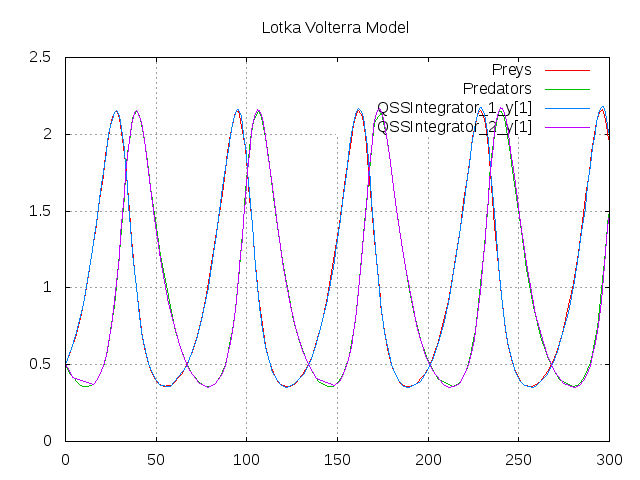
\includegraphics[width=\textwidth]{output/lotka_volterra/lotka_volterra-all.png}
\end{frame}
%%%%%%%%%%%%%%%%%%%%%%%%%%%%%%%%%%%%%%%%%%%%%%%%%%%%%%%%%%%%%%%%%%%%%%%%%%%%%%%

	\subsection{Líneas de Transmisión}
	\subsection{Comparaciones}

%%%%%%%%%%%%%%%%%%%%%%%%%%%%%%%%%%%%%%%%%%%%%%%%%%%%%%%%%%%%%%%%%%%%%%%%%%%%%%%
\begin{frame}{Resultados - Líneas de Transmisión}
\begin{equation*}
\begin{split}
\frac{d v_{j}}{d t} &= \frac{i_{j} - i_{j+1}}{C} \\
\frac{d i_{j}}{d t} &= \frac{v_{j-1} - v_{j}}{L} \\	
\end{split}
\end{equation*}

para $j = 2 \dots N$

Consideramos un pulso de entrada:
\begin{equation*}
v_0(t) = \left\{ 
  \begin{array}{l l}
    1 \text{ si } t < 1 \\
    0 \text{ en caso contrario }
  \end{array} \right.
\end{equation*}
\end{frame}
%%%%%%%%%%%%%%%%%%%%%%%%%%%%%%%%%%%%%%%%%%%%%%%%%%%%%%%%%%%%%%%%%%%%%%%%%%%%%%%

%%%%%%%%%%%%%%%%%%%%%%%%%%%%%%%%%%%%%%%%%%%%%%%%%%%%%%%%%%%%%%%%%%%%%%%%%%%%%%%
\begin{frame}{Resultados - Modelo Líneas de Transmisión en PowerDEVS}
\begin{figure}[H]
 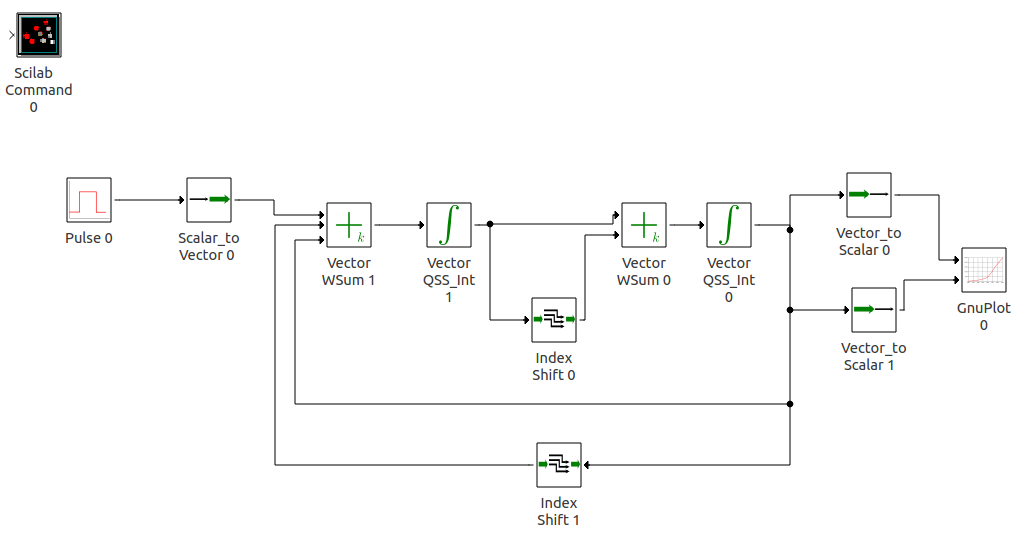
\includegraphics[width=\linewidth]{lclines}
\end{figure}
\end{frame}

\begin{frame}{Resultados - Líneas de Transmisión}
\begin{figure}[H]
\begin{minipage}{0.5\textwidth}
\centering
PowerDEVS\\
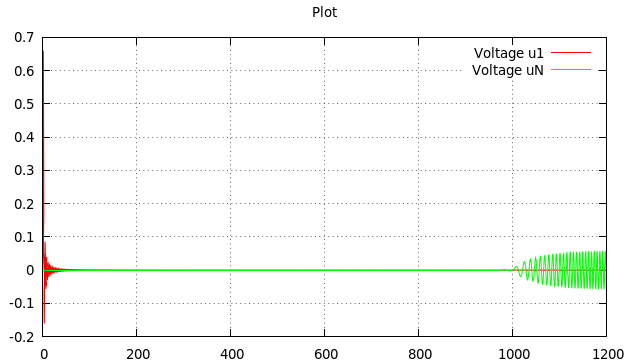
\includegraphics[width=\linewidth]{lcline-pd}
\end{minipage}\hfill\begin{minipage}{0.5\textwidth}
\centering
QSS-Solver\\
 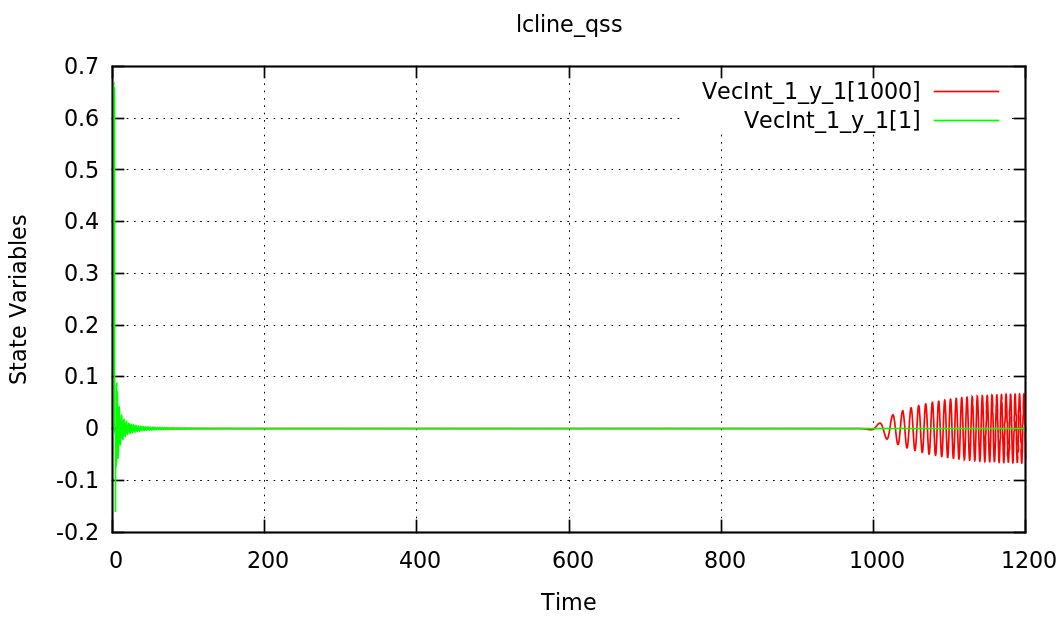
\includegraphics[width=\linewidth]{lcline-qss}
\end{minipage}
\end{figure}
\end{frame}
%%%%%%%%%%%%%%%%%%%%%%%%%%%%%%%%%%%%%%%%%%%%%%%%%%%%%%%%%%%%%%%%%%%%%%%%%%%%%%%

%%%%%%%%%%%%%%%%%%%%%%%%%%%%%%%%%%%%%%%%%%%%%%%%%%%%%%%%%%%%%%%%%%%%%%%%%%%%%%%
\begin{frame}{Resultados - Líneas de Transmisión}
 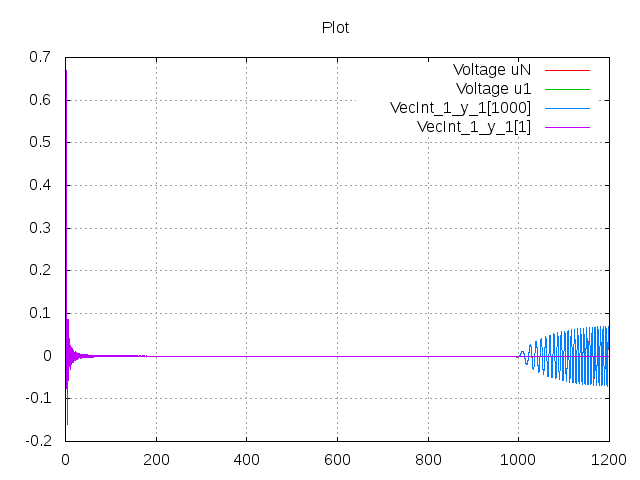
\includegraphics[width=\linewidth]{output/lcline/lcline-all}
\end{frame}
%%%%%%%%%%%%%%%%%%%%%%%%%%%%%%%%%%%%%%%%%%%%%%%%%%%%%%%%%%%%%%%%%%%%%%%%%%%%%%%

%%%%%%%%%%%%%%%%%%%%%%%%%%%%%%%%%%%%%%%%%%%%%%%%%%%%%%%%%%%%%%%%%%%%%%%%%%%%%%%
\begin{frame}{Resultados - Resumen}
\scalebox{0.8}{%
\begin{tabular}{lrrr}
\toprule
{\bf Modelos}            &  {\bf P.DEVS(ms)} & {\bf QSS-S. (ms)} & {\bf Mejora (\%)} \\
\toprule
Lotka  Voltera       		& 11            & 2         & 81 \\
Lineas de Transmisión      & 76402         & 34982         & 54          \\
Inversores(LIQSS2)    	& 25046         & 7694         & 69        \\
ADR(LIQSS2)  		& 6089          & 568         & 90        \\
Convertidor de Voltaje     	& 268           & 10         & 96         

\end{tabular}
}
\end{frame}
%%%%%%%%%%%%%%%%%%%%%%%%%%%%%%%%%%%%%%%%%%%%%%%%%%%%%%%%%%%%%%%%%%%%%%%%%%%%%%%

\section{Conclusiones}

%%%%%%%%%%%%%%%%%%%%%%%%%%%%%%%%%%%%%%%%%%%%%%%%%%%%%%%%%%%%%%%%%%%%%%%%%%%%%%%
\begin{frame}{Conclusiones}
\begin{itemize}
\item<1-> Realizamos una herramienta que traduce modelos PowerDEVS a modelos $\mu$-Modelica, que pueden ser ejecutados en QSS-Solver. 
\item<2-> Para lo cual se generaron de forma manual los modelos Modelica equivalentes a los bloques PowerDEVS utilizados en los ejemplos.
\item<3-> Se desarrolló un algoritmo de traducción para la estructura de archivos PDS de PowerDEVS sin modelos acoplados.
\item<4-> Se desarrolló un algoritmo para el aplanado de modelos PowerDEVS.
\item<5-> Se implementaron transformaciones automáticas sobre el código Modelica para utilizar QSS-Solver.
\item<6-> Se logró una mejora del tiempo de simulación las cuales alcanzan cerca del 90 \% en modelos grandes.
\item<7-> Mostramos además cómo se mantienen los valores obtenidos de la simulación.
\end{itemize}
\end{frame}
%%%%%%%%%%%%%%%%%%%%%%%%%%%%%%%%%%%%%%%%%%%%%%%%%%%%%%%%%%%%%%%%%%%%%%%%%%%%%%%

%%%%%%%%%%%%%%%%%%%%%%%%%%%%%%%%%%%%%%%%%%%%%%%%%%%%%%%%%%%%%%%%%%%%%%%%%%%%%%%
\begin{frame}{Trabajos Futuros}
\begin{itemize}
\item Para poder convertir una mayor variedad de modelos de PowerDEVS, es necesario escribir más modelos en Modelica equivalentes a los modelos atómicos.
\item Algunos modelo atómicos necesitan expandir el QSS-Solver para poder ser ejecutados, por ejemplo los modelos de tiempo real.
\item La librería modelicacc , ha sido actualizada con un nuevo \quotes{parser}.
\item La expansión de variables vectoriales, donde los valores provienen de expresiones del entorno Scilab es siempre tratado como un valor escalar y no como uno vectorial. 
\item Es deseable que podamos llamar a esta conversión desde el mismo PowerDEVS y ejecutar el modelo resultante en el QSS-Solver.
\end{itemize}
\end{frame}
%%%%%%%%%%%%%%%%%%%%%%%%%%%%%%%%%%%%%%%%%%%%%%%%%%%%%%%%%%%%%%%%%%%%%%%%%%%%%%%

%%%%%%%%%%%%%%%%%%%%%%%%%%%%%%%%%%%%%%%%%%%%%%%%%%%%%%%%%%%%%%%%%%%%%%%%%%%%%%%
\begin{frame}
\Huge{\centerline{¿Preguntas?}}
\end{frame}
%%%%%%%%%%%%%%%%%%%%%%%%%%%%%%%%%%%%%%%%%%%%%%%%%%%%%%%%%%%%%%%%%%%%%%%%%%%%%%%

%%%%%%%%%%%%%%%%%%%%%%%%%%%%%%%%%%%%%%%%%%%%%%%%%%%%%%%%%%%%%%%%%%%%%%%%%%%%%%%
\begin{frame}
\Huge{\centerline{Gracias!}}
\end{frame}
%%%%%%%%%%%%%%%%%%%%%%%%%%%%%%%%%%%%%%%%%%%%%%%%%%%%%%%%%%%%%%%%%%%%%%%%%%%%%%%



\end{document}

